\documentclass[12pt]{article}
\usepackage[brazil]{babel}
\usepackage{sbc-template}
\usepackage{graphicx,url}
\usepackage[utf8]{inputenc}

\usepackage[hidelinks]{hyperref}
\usepackage{amsmath}
\usepackage{booktabs}
\usepackage{float}



\sloppy

\title{Análise de Sentimento com Dados Sintéticos Gerados por LLMs: Avaliação Cross-Domain em Dois Nichos}

\author{Davi Romauski Meurer\inst{1}, Marlon Marcon\inst{1}}

\address{Departamento de Engenharia de Software\\
  Universidade Tecnológica Federal do Paraná (UTFPR) -- Dois Vizinhos, PR -- Brasil
  \email{davimeurer@alunos.utfpr.edu.br, marlonmarcon@utfpr.edu.br}
}

\begin{document}

\maketitle

\begin{abstract}
The lack of labeled datasets in Brazilian Portuguese is a very common obstacle for sentiment analysis research. This work evaluates whether synthetic data generated by three LLMs — ChatGPT, Gemini, and Claude — can be used to train classifiers in a real-world scenario. Two synthetic datasets of 1,800 sentences each were built (movies and series, and mobile apps), and five classifiers (Naive Bayes, Logistic Regression, Linear SVM, LSTM, and BERTimbau) were trained and evaluated under five methodological views: synthetic to synthetic, real to real with controlled volume, synthetic to real with controlled volume, real to real with natural unbalanced distribution, and synthetic to real with natural unbalanced distribution. The results show that the synthetic to synthetic scenario reaches 97\% F1 with BERTimbau, but the synthetic to real cross-domain test caps at 47\% in the movies and series niche and 80\% in the apps niche. The 33-point difference in the movies and series category persists even when tripling the synthetic training volume, which indicates that the limitation comes from a structural difference in distribution between LLM-generated text and reviews written by real users, and not from data scarcity. The large difference between the two niches suggests that the viability of synthetic data depends on how regular and objective the evaluation domain is.
\end{abstract}

\begin{resumo}
A falta de datasets rotulados em português brasileiro é um obstáculo muito comum para pesquisas em análise de sentimento. Este trabalho avalia se dados sintéticos gerados por três LLMs — ChatGPT, Gemini e Claude — podem ser usados para treinar classificadores em um cenário real. Foram construídos dois datasets sintéticos de 1.800 frases cada (filmes e séries, e aplicativos móveis), e foram treinados cinco classificadores (Naive Bayes, Regressão Logística, SVM Linear, LSTM e BERTimbau) avaliados em cinco visões metodológicas: sintético para sintético, real para real com volume controlado, sintético para real com volume controlado, real para real com distribuição natural desbalanceada e sintético para real com distribuição natural desbalanceada. Os resultados mostram que o cenário sintético para sintético chega a 97\% de F1 com BERTimbau, mas o teste cross-domain sintético para real fica em no máximo 47\% no nicho de filmes e séries e 80\% no nicho de aplicativos. A diferença de 33 pontos na categoria de filmes e séries se mantém mesmo triplicando o volume de treino sintético, o que indica que a limitação vem de uma diferença estrutural na distribuição entre texto gerado por LLMs e reviews escritas por usuários reais, e não da escassez de dados. A diferença grande entre os dois nichos sugere que a viabilidade dos dados sintéticos depende de quão regular e objetivo é o domínio de avaliação.
\end{resumo}


% ====================================================================
% SEÇÃO 1 — INTRODUÇÃO
% ====================================================================

\section{Introdução}

A análise de sentimento é uma tarefa de classificação de texto que busca identificar a polaridade — positiva, negativa ou neutra — de uma opinião dita em linguagem natural. Tem aplicações diretas em mineração de opinião, monitoramento de redes sociais e análise de feedback de produtos e serviços \cite{jm3}. Treinar modelos para essa tarefa, no entanto, depende de datasets rotulados de qualidade, e a construção manual desses datasets é cara, demorada e suscetível a inconsistências. Esse problema é ainda mais notado quando vamos para o cenário do idioma português brasileiro, onde a disponibilidade de recursos linguísticos anotados é bem menor do que no inglês \cite{souza2022brazilian}.

Uma maneira que vem sendo cada vez mais cogitada e chamando atenção é o uso de grandes modelos de linguagem artificial (LLMs) como geradores de dados sintéticos de treinamento \cite{liu2024best, nadas2025synthetic}. Modelos como ChatGPT, Gemini e Claude conseguem produzir textos coerentes e contextualmente adequados em português, o que abre a possibilidade de criar datasets rotulados sem depender de inserção ou classificação humana em plataformas de avaliação. Trabalhos recentes já investigaram essa abordagem para classificação de texto e análise de sentimento baseada em aspectos, com resultados promissores em cenários de poucos recursos \cite{li2023synthetic, hellwig2025exploring}.

Este trabalho investiga três perguntas relacionadas. A primeira é qual a assertividade de classificadores treinados exclusivamente com dados sintéticos. A segunda é se há coerência entre os dados produzidos por diferentes LLMs geradores. A terceira é se modelos treinados em dados sintéticos generalizam para dados reais (avaliação cross-domain). Para responder essas perguntas, foram construídos dois datasets sintéticos de 1.800 frases cada, em dois nichos distintos: críticas de filmes e séries (com base no UTLC-Movies) e reviews de aplicativos móveis (com base no UTLC-Apps). Cinco classificadores foram avaliados sob cinco visões metodológicas, cobrindo desde modelos lineares com TF-IDF (Naive Bayes, Regressão Logística e SVM Linear) até arquiteturas neurais (LSTM e BERTimbau).

Este artigo está organizado da seguinte forma: a Seção~\ref{sec:fundamentacao} apresenta a fundamentação teórica. A Seção~\ref{sec:relacionados} revisa trabalhos relacionados. A Seção~\ref{sec:metodologia} descreve a metodologia, incluindo a definição das cinco visões e os dois nichos. A Seção~\ref{sec:resultados} apresenta os resultados organizados em três blocos: domínio sintético, domínio real e cross-domínio. Por fim, a Seção~\ref{sec:conclusao} traz as conclusões.


% ====================================================================
% SEÇÃO 2 — FUNDAMENTAÇÃO TEÓRICA
% ====================================================================

\section{Fundamentação Teórica}
\label{sec:fundamentacao}

A análise de sentimento pode ser considerada como um problema de classificação supervisionada, onde o objetivo é atribuir uma classe (Positiva, Negativa ou Neutra) a cada instância textual \cite{jm3}. Neste trabalho a classificação é feita no nível da sentença. Um dos desafios conhecidos da tarefa é o tratamento de negações compostas e ambiguidades — frases como ``não gostei nada desse filme'' têm polaridade oposta ao que seria esperado pela presença isolada do verbo ``gostar'', e esse tipo de construção tende a causar erros em classificadores baseados apenas em frequência de termos.

Para que algoritmos processem texto, é preciso converter as frases em representações numéricas. O TF-IDF (\textit{Term Frequency–Inverse Document Frequency}) representa cada documento como um vetor que ajusta as contagens de palavras pela frequência inversa delas no corpus, penalizando termos muito frequentes — como preposições — que aparecem em quase todos os documentos \cite{rossi2019}. Os classificadores clássicos utilizados neste trabalho operam sobre essa representação: o Naive Bayes Multinomial é um modelo probabilístico que assume independência condicional entre os atributos, a Regressão Logística é um classificador discriminativo que aprende diretamente a fronteira de decisão, e o SVM Linear busca o hiperplano de máxima margem entre as classes \cite{pang2002}.

Para os modelos avançados, o trabalho utiliza dois paradigmas distintos. O LSTM (\textit{Long Short-Term Memory}) é uma rede neural recorrente que processa as palavras em sequência, com embeddings aprendidos do zero a partir do dataset de treino. Já o BERTimbau \cite{souza2022brazilian} é um modelo BERT pré-treinado em 2,7 bilhões de palavras de português brasileiro, baseado na arquitetura Transformer. O modelo foi pré-treinado pela equipe da NeuralMind/USP em tarefas de \textit{Masked Language Modeling}, ou seja, ele não foi originalmente treinado para análise de sentimento. Neste trabalho, o BERTimbau é adaptado para a tarefa via fine-tuning: as cabeças de predição do pré-treino são removidas e uma camada linear de classificação é adicionada e treinada com os dados sintéticos.

Para avaliar os classificadores, são utilizadas cinco métricas: acurácia (proporção de classificações corretas sobre o total), precisão (proporção de verdadeiros positivos entre as predições positivas), recall (proporção de verdadeiros positivos entre os exemplos reais de uma classe), F1-Score weighted (média harmônica de precisão e recall ponderada pelo número de amostras por classe) e F1-Score macro (média harmônica simples por classe). A diferença entre F1 weighted e F1 macro é especialmente importante em datasets desbalanceados — o weighted tende a favorecer a classe majoritária, enquanto o macro força o modelo a apresentar bom desempenho em todas as classes igualmente.


% ====================================================================
% SEÇÃO 3 — TRABALHOS RELACIONADOS
% ====================================================================

\section{Trabalhos Relacionados}
\label{sec:relacionados}

Esta seção revisa trabalhos que abordam análise de sentimento com aprendizado de máquina, com foco em aplicações em língua portuguesa e no uso de dados sintéticos para treinamento de classificadores.

\subsection{Análise de Sentimento com Aprendizado de Máquina}

O trabalho pioneiro de \cite{pang2002} estabeleceu que abordagens baseadas em aprendizado de máquina — especialmente Naive Bayes, SVM e Máxima Entropia — superam métodos baseados em regras para classificação de sentimento em resenhas de filmes. Os autores utilizaram o corpus de críticas do IMDb e observaram que o SVM com representação unigrama atingiu cerca de 82,9\% de acurácia, enquanto o Naive Bayes apresentou desempenho competitivo com menor custo computacional.

No contexto brasileiro, \cite{kansaon2019} realizaram análise de sentimento em tweets em português com múltiplas variantes do Naive Bayes e reportaram acurácias entre 79\% e 85\%. \cite{souza2021} propuseram um sistema em tempo real para notícias do mercado financeiro em português, utilizando TF-IDF combinado com Naive Bayes, e atingiram acurácia de 76,8\%. \cite{rossi2019} comparou classificadores como Regressão Logística, Naive Bayes, SVM linear e Random Forest sobre representações BoW e TF-IDF e demonstrou que o TF-IDF apresenta ganhos consistentes sobre o BoW na maioria dos cenários. \cite{souza2022brazilian} unificaram cinco datasets de análise de sentimento em português brasileiro e evidenciaram a escassez de recursos anotados para o idioma.

\subsection{Dados Sintéticos e LLMs para Geração de Dados de Treinamento}

A utilização de dados sintéticos gerados por LLMs para treinamento de modelos é uma área recente. \cite{zhang2024sentiment} avaliaram o desempenho de LLMs em tarefas de análise de sentimento e indicaram que os modelos vão bem em classificação simples de polaridade, mas ficam atrás em tarefas que exigem compreensão mais profunda como detecção de ironia. \cite{hellwig2025exploring} usaram GPT-3.5-turbo e Llama-3-70B para gerar dados anotados para análise baseada em aspectos em cenários de poucos recursos, e mostraram que mesmo pequenas quantidades de dados sintéticos podem complementar datasets escassos. \cite{li2023synthetic} avaliaram a geração de dados com GPT-3.5-Turbo para classificação de texto e reportaram que a efetividade varia conforme a subjetividade da tarefa.

Do ponto de vista metodológico, \cite{liu2024best} compilaram boas práticas para uso de dados sintéticos no treinamento de modelos de linguagem, incluindo técnicas de filtragem e refinamento iterativo, além de discutir riscos como amplificação de viés. \cite{nadas2025synthetic} apresentaram um survey recente sobre o tema e destacaram que a abordagem é especialmente promissora para tarefas com poucos recursos em idiomas que não o inglês. \cite{araujo2024chatgpt} investigaram especificamente as capacidades do ChatGPT para análise de sentimento zero-shot em português brasileiro e demonstraram que o modelo se destaca na determinação de polaridade.

\subsection{Posicionamento deste Trabalho}

A maioria dos trabalhos revisados utiliza LLMs como classificadores diretos em cenários zero-shot ou few-shot, e não como geradores de dados de treinamento para modelos próprios. Além disso, a maior parte foca no inglês e usa um único LLM como fonte. Este trabalho se diferencia em quatro aspectos: utiliza dados 100\% sintéticos gerados por três LLMs distintos (ChatGPT, Gemini e Claude), foca em português brasileiro, avalia explicitamente o cross-domain comparando treino sintético com teste em dados reais, e analisa dois nichos diferentes (filmes e séries, e aplicativos móveis) para entender em que contextos a abordagem é mais ou menos viável.


% ====================================================================
% SEÇÃO 4 — METODOLOGIA
% ====================================================================

\section{Metodologia}
\label{sec:metodologia}

Esta seção descreve o pipeline completo do trabalho, desde a definição das classes e geração dos datasets sintéticos até o protocolo de avaliação. A Seção~\ref{sec:visoes} introduz as cinco visões metodológicas que estruturam toda a análise dos resultados.

\subsection{Definição das Classes de Sentimento}

Antes de gerar os dados, as três classes de sentimento foram definidas explicitamente para que os prompts enviados aos LLMs fossem precisos o suficiente. A classe Positiva contempla textos que expressam satisfação, admiração ou recomendação. A classe Negativa abrange insatisfação, desapontamento ou desaprovação. A classe Neutra compreende textos com informações factuais — sinopses, descrição técnica, dados objetivos — sem emitir juízo de valor.

\subsection{Construção dos Datasets Sintéticos}

Os datasets foram construídos a partir de dados gerados por três LLMs: ChatGPT (OpenAI), Gemini (Google) e Claude (Anthropic). A escolha por múltiplos modelos teve como objetivo reduzir o viés de geração associado a uma única fonte. Para cada LLM foram solicitadas 200 frases por classe via prompts padronizados enviados manualmente pelas interfaces web, totalizando 1.800 frases por nicho (3 LLMs × 3 classes × 200 frases).

O trabalho utiliza dois nichos: filmes e séries (com referência ao UTLC-Movies para os dados reais) e aplicativos móveis (com referência ao UTLC-Apps). Os prompts são isomorfos entre os dois nichos — a única diferença é a substituição de ``filmes e séries'' por ``aplicativos móveis'' e ``espectador'' por ``usuário'', mantendo o resto idêntico. Essa decisão garante que diferenças observadas nos resultados possam ser atribuídas ao nicho e não ao prompt.

A Tabela~\ref{tab:comprimento} mostra o comprimento médio das frases por LLM em cada nicho. ChatGPT é consistente nos dois nichos, com média próxima de 50 caracteres. Claude se adapta ao domínio: 94 caracteres em filmes e séries (frases mais narrativas) e 65 em apps (mais técnicas). Gemini fica em uma posição intermediária. A Figura~\ref{fig:comprimento} apresenta a distribuição completa.

\begin{table}[h]
\centering
\caption{Comprimento médio das frases sintéticas por LLM e nicho (caracteres).}
\label{tab:comprimento}
\begin{tabular}{lccc}
\toprule
\textbf{Nicho} & \textbf{ChatGPT} & \textbf{Claude} & \textbf{Gemini} \\
\midrule
Filmes (Movies) & 49 & 94 & 58 \\
Apps            & 50 & 65 & 66 \\
\bottomrule
\end{tabular}
\end{table}

\begin{figure}[H]
\centering
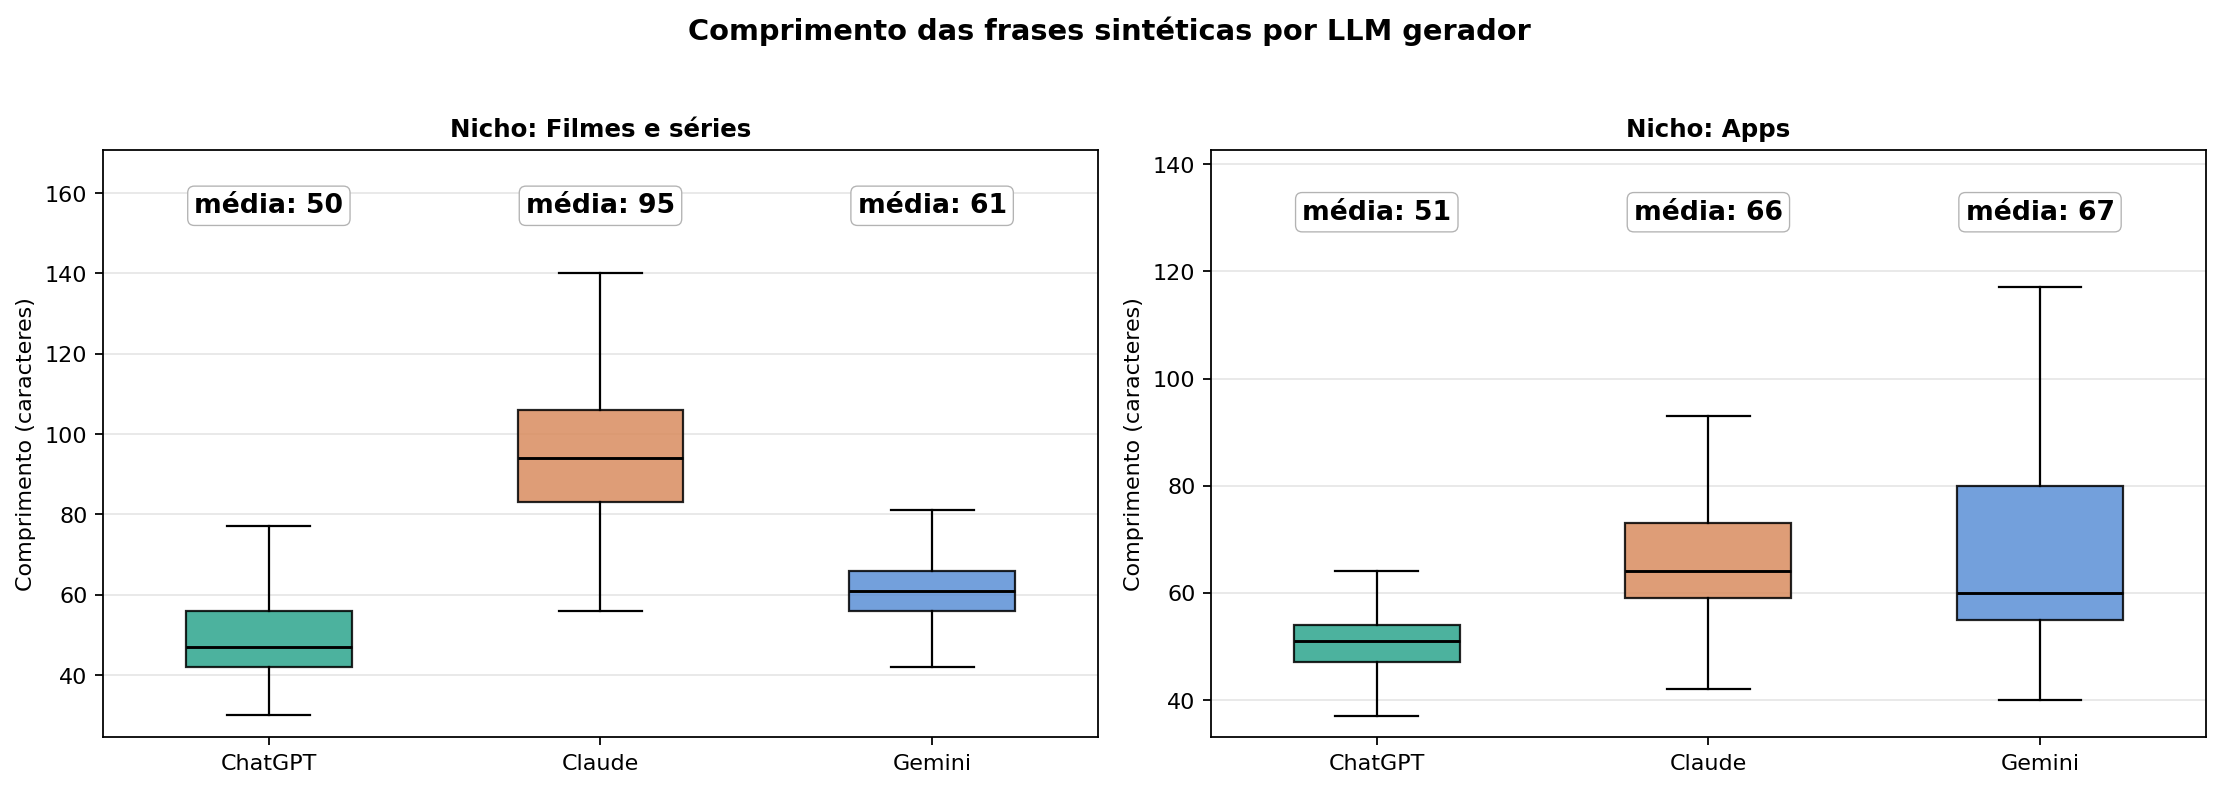
\includegraphics[width=.95\textwidth]{imagens/comprimento_frases_por_llm.png}
\caption{Boxplot do comprimento das frases sintéticas por LLM gerador em cada nicho.}
\label{fig:comprimento}
\end{figure}

\subsection{Dados Reais para Validação Cross-Domain}

Para os experimentos cross-domain, foram utilizados subconjuntos do dataset \texttt{ptbr-sentiment-analysis-datasets} \cite{souza2022brazilian} disponível no Kaggle. Cada nicho usou seu arquivo correspondente (\texttt{utlc\_movies.csv} e \texttt{utlc\_apps.csv}), com aproximadamente 100 mil reviews por nicho carregadas via \texttt{kagglehub}. O dataset original traz a coluna \texttt{rating} com notas de 1 a 5, que foi mapeada para as três classes do trabalho: ratings 4 e 5 viraram Positiva, 1 e 2 viraram Negativa e 3 virou Neutra. A distribuição natural após o mapeamento ficou bastante desbalanceada — em filmes e séries, 71\% Positiva, 20\% Neutra e 9\% Negativa; em apps, 72\% Positiva, 21\% Negativa e 7\% Neutra.

\subsection{As Cinco Visões Metodológicas}
\label{sec:visoes}

A análise é estruturada em cinco visões que combinam a fonte do treino (sintético ou real), a fonte do teste (sintético ou real) e o regime de volume (controlado em 200 frases por classe ou natural desbalanceado). A Tabela~\ref{tab:visoes} resume a configuração de cada uma.

\begin{table}[h]
\centering
\caption{Configuração das cinco visões metodológicas.}
\label{tab:visoes}
\small
\begin{tabular}{cllc}
\toprule
\textbf{Visão} & \textbf{Treino} & \textbf{Teste} & \textbf{Volume} \\
\midrule
V1 & Sintético & Sintético & 600/classe (controlado) \\
V2 & Real      & Real      & 600/classe (controlado) \\
V3 & Sintético & Real      & 600/classe (mesmo test set do V2) \\
V4 & Real      & Real      & Natural desbalanceado (~80k/classe) \\
V5 & Sintético & Real      & Sint. controlado, real desbalanceado (mesmo test set do V4) \\
\bottomrule
\end{tabular}
\end{table}

A escolha por usar o mesmo conjunto de teste em V2 e V3 é uma decisão de controle experimental: como o conjunto de teste é idêntico, a única variável que muda entre as duas visões é a fonte do treino. O mesmo vale para V4 e V5. Esse desenho permite isolar o efeito do uso de dados sintéticos no desempenho final.

\subsection{Modelos de Classificação}

Foram avaliados cinco classificadores. Os três clássicos foram implementados via scikit-learn \cite{pedregosa2011} com hiperparâmetros padrão: Naive Bayes Multinomial (\texttt{MultinomialNB()}), Regressão Logística (\texttt{LogisticRegression(max\_iter=1000)}) e SVM Linear (\texttt{LinearSVC(max\_iter=5000)}). O LSTM foi implementado em PyTorch com uma camada recorrente de 128 unidades, embeddings aprendidos do zero (dimensão 128), dropout de 0,3 e otimizador AdamW com taxa de aprendizado $1\mathrm{e}{-3}$. O BERTimbau \cite{souza2022brazilian} foi utilizado em sua versão base (\texttt{neuralmind/bert-base-portuguese-cased}), com fine-tuning por 3 epochs, batch size de 16, taxa de aprendizado $2\mathrm{e}{-5}$ e tamanho máximo de sequência de 128 tokens.

Para todas as visões usou-se semente aleatória fixa (\texttt{random\_state=42}) para garantir reprodutibilidade. Os experimentos com BERT e LSTM foram executados em GPU NVIDIA T4 via Google Colab, com tempo total de aproximadamente 50 minutos para o nicho de filmes e séries, e 35 minutos para o nicho de apps.

\subsection{Pré-processamento e Vetorização}

Os textos sintéticos passaram por quatro operações de limpeza: conversão para minúsculas, remoção de pontuação e caracteres especiais, normalização de espaços e remoção de duplicatas. Para os modelos clássicos, a vetorização foi feita com \texttt{TfidfVectorizer} do scikit-learn (parâmetros padrão, sem remoção explícita de stopwords). Para o LSTM, a tokenização foi por palavra (split em espaço) com vocabulário construído a partir do treino de cada visão. Para o BERTimbau, foi usado o tokenizer próprio do modelo (\texttt{AutoTokenizer.from\_pretrained}).

\subsection{Ambiente Experimental}

Os experimentos foram implementados em Python 3, com scikit-learn \cite{pedregosa2011}, pandas, matplotlib, PyTorch e Hugging Face Transformers. O código foi estruturado em notebooks Jupyter com detecção automática de ambiente (Google Colab ou execução local). O repositório está disponível em \url{https://github.com/ROMAUSKI/tcc-analise-sentimento}.


% ====================================================================
% SEÇÃO 5 — RESULTADOS E DISCUSSÃO
% ====================================================================

\section{Resultados e Discussão}
\label{sec:resultados}

Esta seção apresenta os resultados organizados em três blocos principais: o desempenho no domínio sintético (V1), no domínio real (V2 e V4) e no cross-domínio entre os dois (V3 e V5). Em seguida são apresentados o comparativo entre os dois nichos e a validação cruzada do dataset original. Os valores reportados nas tabelas a seguir referem-se ao F1-Score weighted (e ao F1-Score macro nas visões desbalanceadas V4 e V5, onde a diferença entre as duas métricas é informativa). Os gráficos completos com as cinco métricas estão disponíveis em \url{https://github.com/ROMAUSKI/tcc-analise-sentimento/tree/main/resultados}.

\subsection{Domínio Sintético (V1)}

A primeira visão avalia os modelos treinados e testados em dados sintéticos do mesmo nicho. A Tabela~\ref{tab:v1} mostra que os cinco modelos atingem F1-Score acima de 80\% em ambos os nichos, e o BERTimbau alcança 97\% em filmes e séries, e 97\% em apps. Esse resultado mostra que os dados sintéticos gerados pelos LLMs são internamente coerentes — quando o modelo é avaliado em frases do mesmo tipo que viu no treino, a classificação é praticamente perfeita.

\begin{table}[h]
\centering
\caption{F1-Score weighted (\%) na visão V1: Sintético $\rightarrow$ Sintético.}
\label{tab:v1}
\begin{tabular}{lcc}
\toprule
\textbf{Modelo} & \textbf{Filmes} & \textbf{Apps} \\
\midrule
Naive Bayes         & 88,07 & 88,82 \\
Regressão Logística & 86,93 & 89,69 \\
SVM Linear          & 88,33 & 91,07 \\
LSTM                & 81,40 & 85,22 \\
BERTimbau           & 97,49 & 97,22 \\
\bottomrule
\end{tabular}
\end{table}

Esse resultado, no entanto, precisa ser lido com cautela. O alto desempenho em V1 não significa que os classificadores funcionariam bem em produção — significa apenas que os modelos aprenderam o padrão dos dados sintéticos, que é mais regular e previsível do que o de avaliações reais. As visões V3 e V5, apresentadas mais adiante, é que realmente testam se esse aprendizado se transfere.

\subsection{Domínio Real (V2 e V4)}

As visões V2 e V4 usam dados reais tanto no treino quanto no teste, com regimes de volume diferentes. V2 é controlada (600 frases por classe) e V4 usa o dataset inteiro com distribuição natural desbalanceada. A Tabela~\ref{tab:v2v4} apresenta os resultados.

\begin{table}[h]
\centering
\caption{F1-Score (\%) nas visões V2 (controlada) e V4 (desbalanceada). Para V4 são reportadas duas métricas porque a distribuição é desbalanceada.}
\label{tab:v2v4}
\small
\begin{tabular}{lcccc}
\toprule
& \multicolumn{2}{c}{\textbf{V2: F1 weighted}} & \multicolumn{2}{c}{\textbf{V4: F1 weighted / F1 macro}} \\
\cmidrule(lr){2-3} \cmidrule(lr){4-5}
\textbf{Modelo} & \textbf{Filmes} & \textbf{Apps} & \textbf{Filmes} & \textbf{Apps} \\
\midrule
Naive Bayes         & 52,10 & 62,50 & 64,36 / 38,48 & 81,16 / 56,13 \\
Regressão Logística & 54,45 & 61,18 & 70,93 / 52,05 & 82,84 / 60,04 \\
SVM Linear          & 54,80 & 58,16 & 70,59 / 51,92 & 82,36 / 59,39 \\
LSTM                & 39,23 & 56,01 & 71,99 / 54,89 & 83,86 / 63,11 \\
BERTimbau           & 60,42 & 66,84 & 76,46 / 62,29 & 86,27 / 66,59 \\
\bottomrule
\end{tabular}
\end{table}

V2 mostra que mesmo com dados reais, classificar reviews em três classes com apenas 600 amostras por classe não é trivial — os modelos clássicos ficam entre 52 e 62\% de F1, e o BERTimbau alcança 60-67\%. V4 mostra um cenário diferente: com o dataset real completo, todos os modelos sobem para 64-86\% no F1 weighted. Essa subida acompanha o que a literatura prevê — mais dados ajudam, especialmente os modelos discriminativos. Mas o F1 macro revela um efeito importante: enquanto o weighted está entre 64 e 86\%, o macro fica entre 38 e 67\%. Essa diferença vem do desbalanceamento natural — a classe Positiva domina (71-72\% das amostras), e o modelo acerta muito nela mas erra mais nas classes minoritárias. O F1 macro, que dá o mesmo peso a cada classe, expõe esse comportamento.

\subsection{Cross-Domínio (V3 e V5)}

As visões V3 e V5 são as mais relevantes do trabalho porque medem se os classificadores treinados com dados sintéticos conseguem generalizar para reviews reais. V3 testa em conjunto controlado (mesmo test set do V2) e V5 testa em conjunto desbalanceado (mesmo test set do V4). A Tabela~\ref{tab:v3v5} apresenta os resultados.

\begin{table}[h]
\centering
\caption{F1-Score (\%) nas visões V3 e V5: Sintético $\rightarrow$ Real.}
\label{tab:v3v5}
\small
\begin{tabular}{lcccc}
\toprule
& \multicolumn{2}{c}{\textbf{V3: F1 weighted}} & \multicolumn{2}{c}{\textbf{V5: F1 weighted / F1 macro}} \\
\cmidrule(lr){2-3} \cmidrule(lr){4-5}
\textbf{Modelo} & \textbf{Filmes} & \textbf{Apps} & \textbf{Filmes} & \textbf{Apps} \\
\midrule
Naive Bayes         & 34,75 & 40,42 & 47,11 / 32,29 & 67,04 / 38,97 \\
Regressão Logística & 38,77 & 40,24 & 45,30 / 32,61 & 64,16 / 36,91 \\
SVM Linear          & 36,45 & 42,17 & 45,47 / 32,50 & 64,42 / 37,05 \\
LSTM                & 34,83 & 31,66 & 42,13 / 27,13 & 59,55 / 36,23 \\
BERTimbau           & 47,10 & 48,21 & 58,95 / 42,62 & 80,95 / 55,68 \\
\bottomrule
\end{tabular}
\end{table}

Comparando V3 com V1 fica claro o tamanho do gap: o BERTimbau cai de 97\% (V1) para 47\% em filmes e séries, e 48\% em apps. Os modelos clássicos caem para 34-42\%. Esse é o reality gap — os classificadores treinados com dados sintéticos não conseguem reproduzir esse desempenho quando o teste vem de avaliações reais. A diferença entre V1 e V3 é de cerca de 50 pontos para o BERTimbau e 50-55 pontos para os modelos clássicos.

A Figura~\ref{fig:comparativo_f1w} mostra o comparativo lado a lado dos dois nichos para todas as visões e todos os modelos, com F1 weighted. O padrão fica visualmente claro: V1 muito alto, V2 e V4 razoáveis, V3 e V5 ruins.

\begin{figure}[H]
\centering
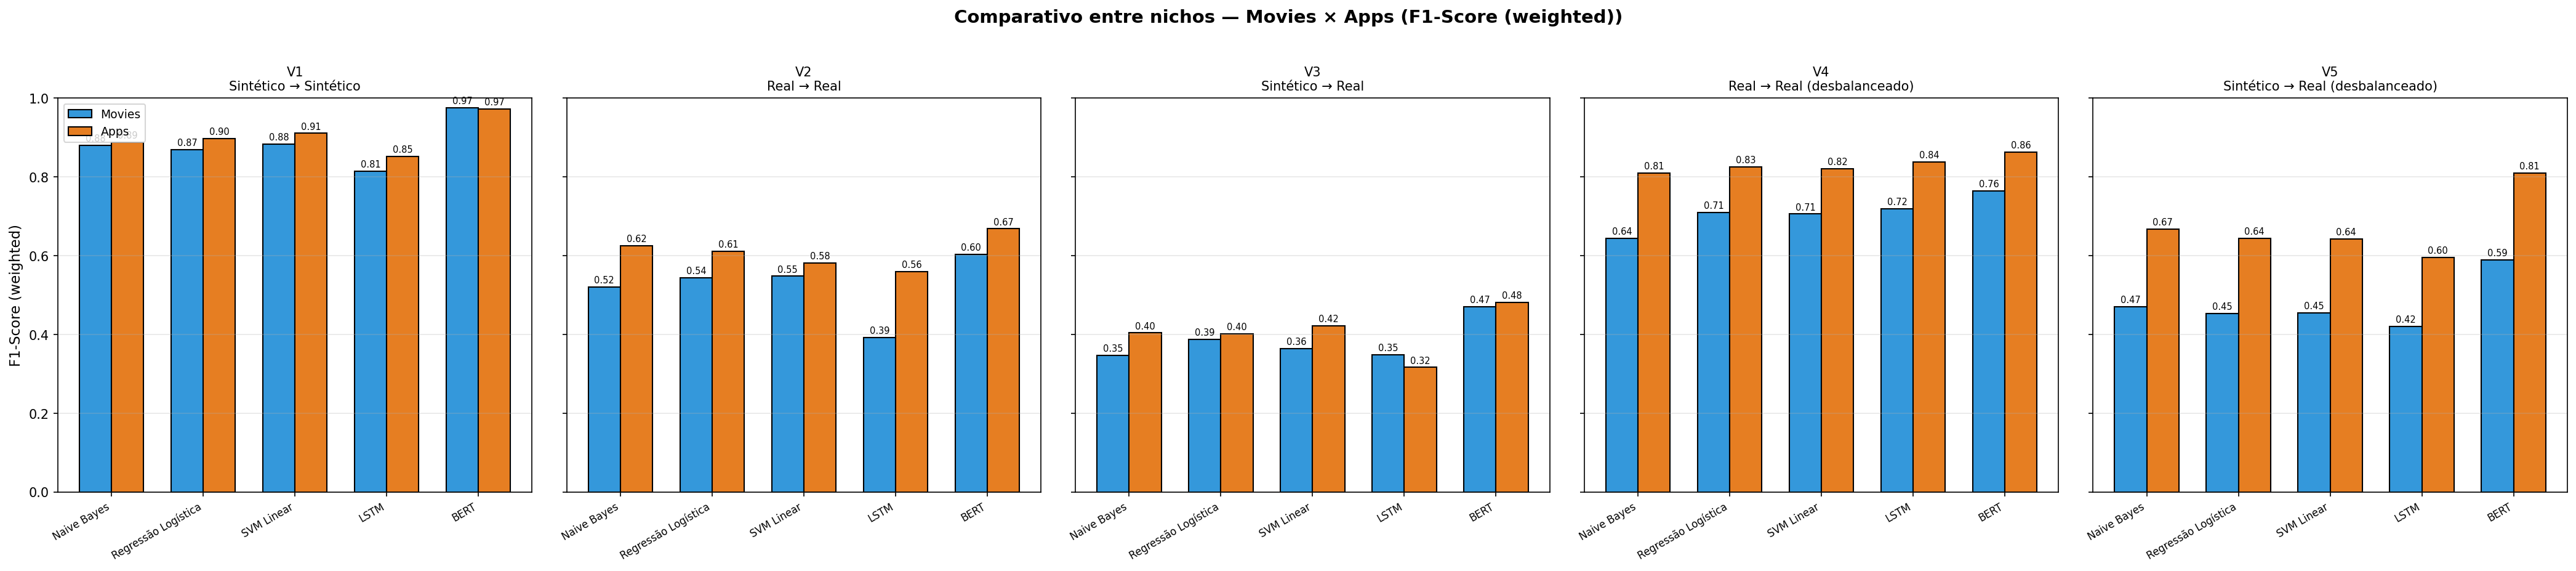
\includegraphics[width=\textwidth]{imagens/comparativo_nichos_f1weighted.png}
\caption{F1-Score weighted nas cinco visões para os dois nichos (Movies e Apps).}
\label{fig:comparativo_f1w}
\end{figure}

A Figura~\ref{fig:comparativo_f1m} mostra o mesmo comparativo para o F1 macro, onde fica evidente o impacto do desbalanceamento em V4 e V5. As demais métricas (acurácia, precisão e recall) seguem padrão similar e estão disponíveis no repositório do trabalho.

\begin{figure}[H]
\centering
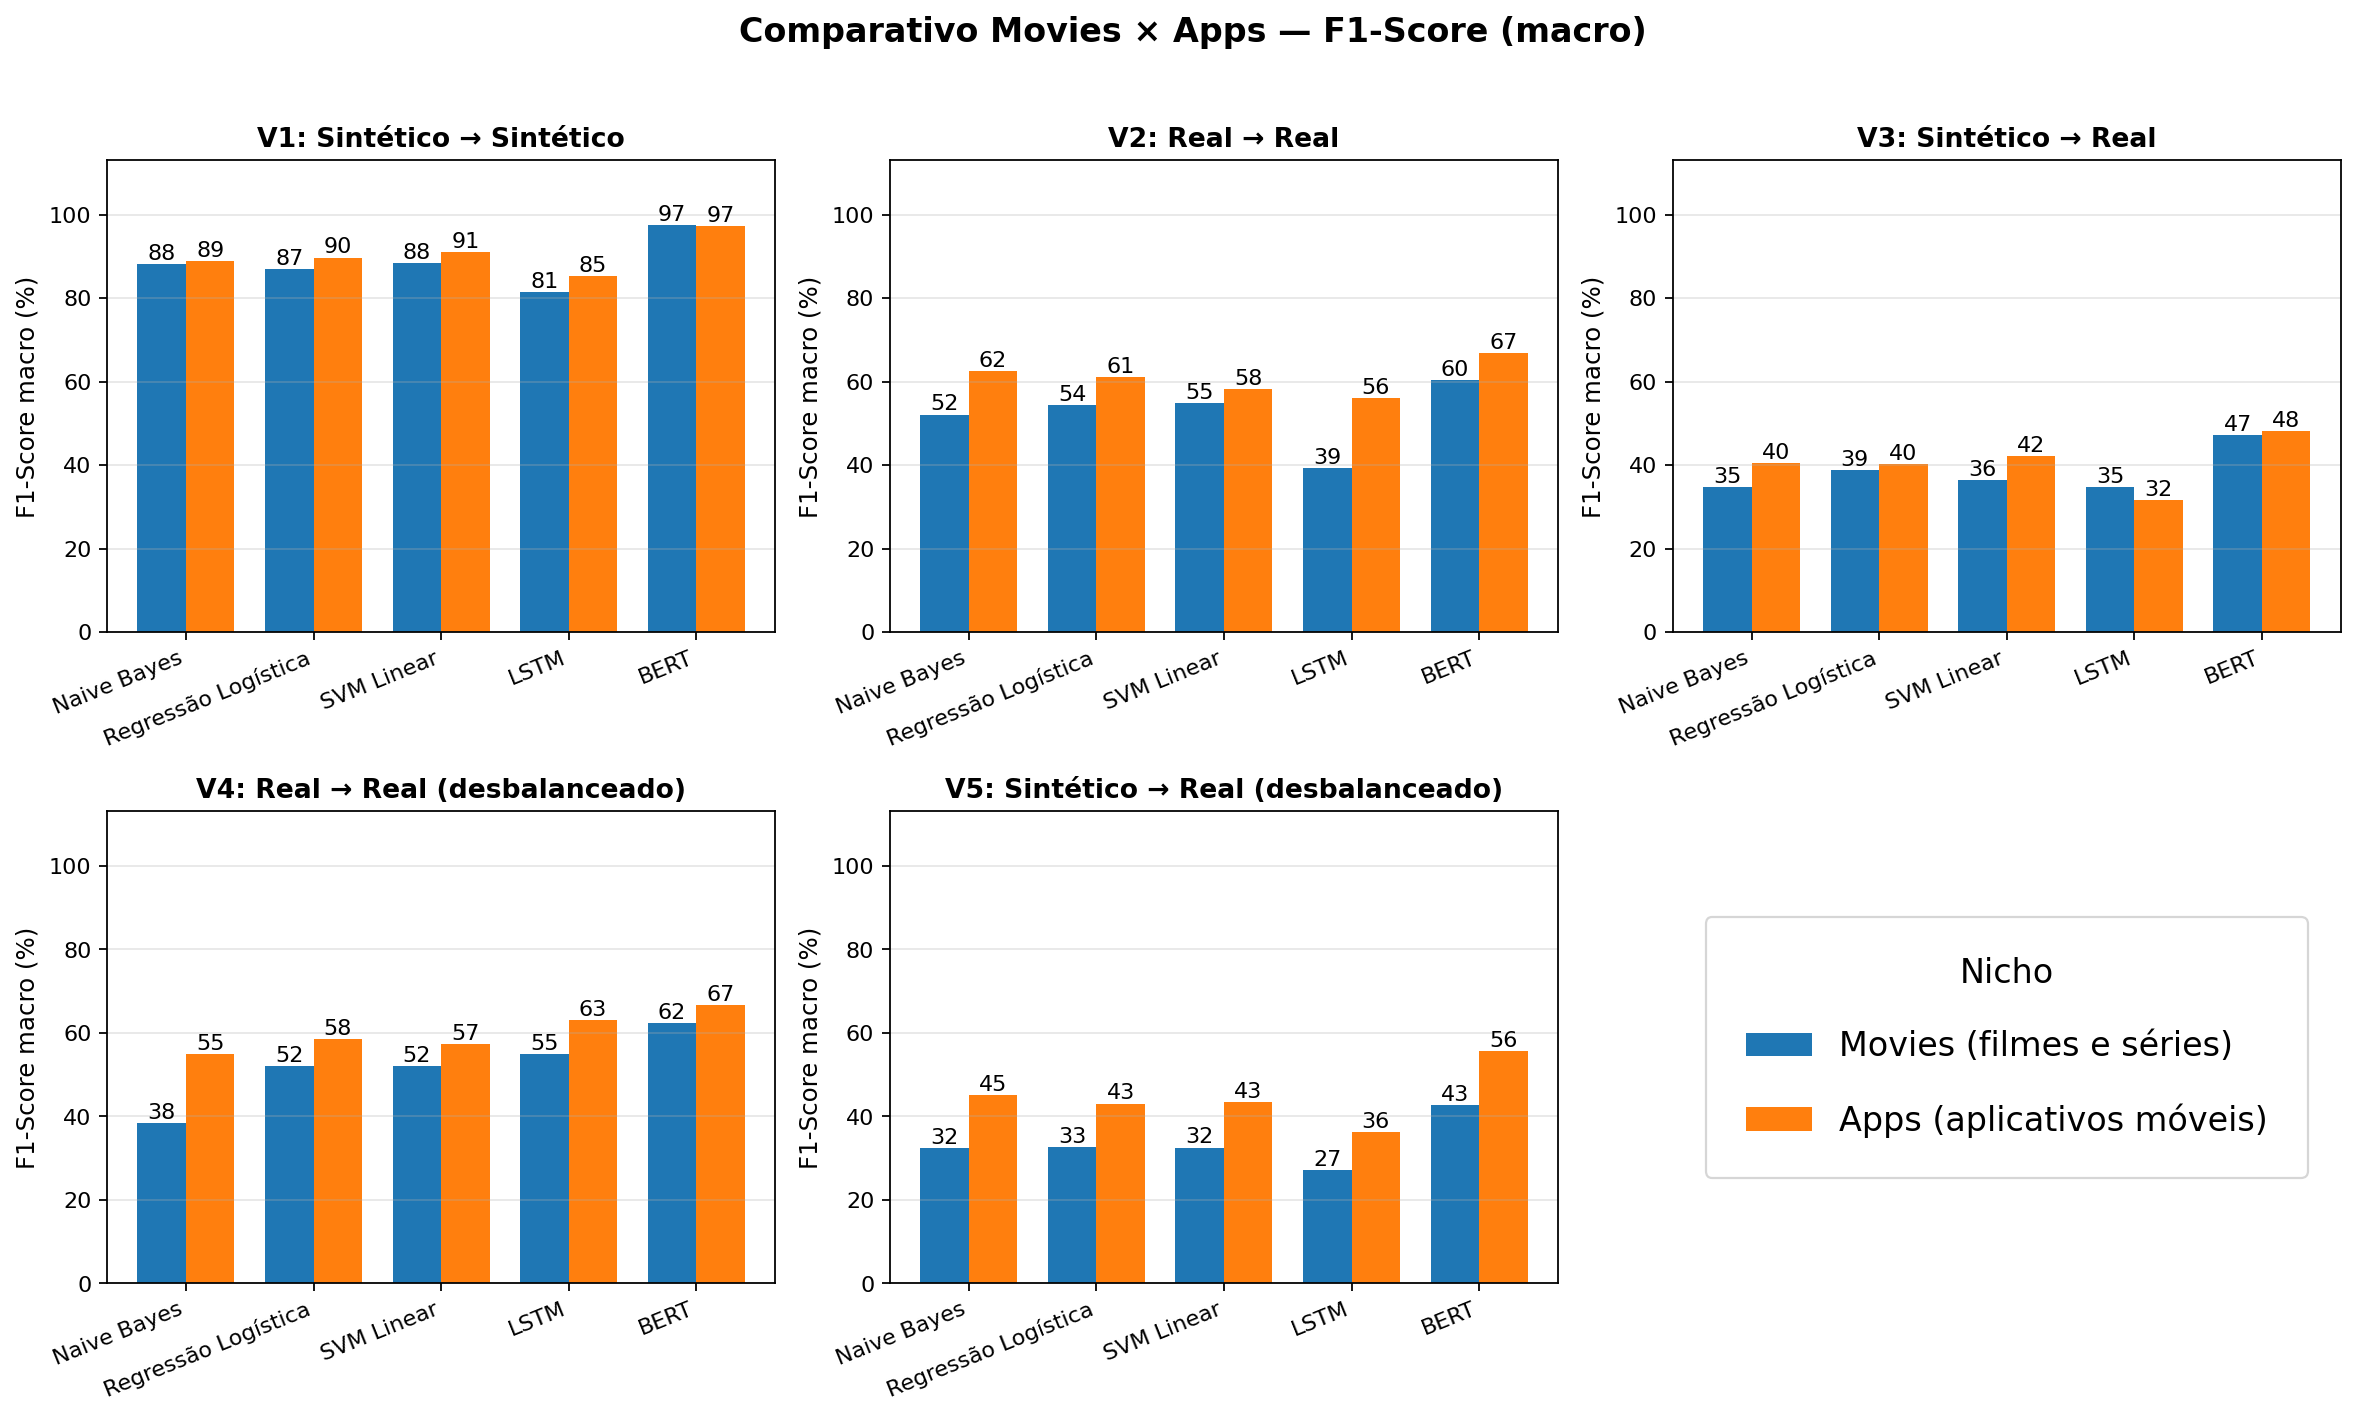
\includegraphics[width=\textwidth]{imagens/comparativo_nichos_f1macro.png}
\caption{F1-Score macro nas cinco visões para os dois nichos. A diferença em relação ao F1 weighted nas visões V4 e V5 expõe o viés de classe majoritária.}
\label{fig:comparativo_f1m}
\end{figure}

Um experimento adicional foi feito para verificar se aumentar o volume de dados sintéticos reduziria o gap. O dataset sintético foi balanceado em duas configurações: 200 frases por classe e 600 frases por classe (triplicando o volume de treino). A Figura~\ref{fig:200vs600} mostra o resultado para o nicho de filmes. Em V1 (sintético-sintético) e V2 (real-real) o desempenho sobe com mais dados, como esperado. Mas em V3 (sintético-real) o desempenho fica praticamente igual nas duas configurações. Isso indica que o gap em V3 não vem da escassez de dados sintéticos — vem de uma diferença estrutural na distribuição entre o texto gerado por LLMs e as reviews reais.

\begin{figure}[H]
\centering
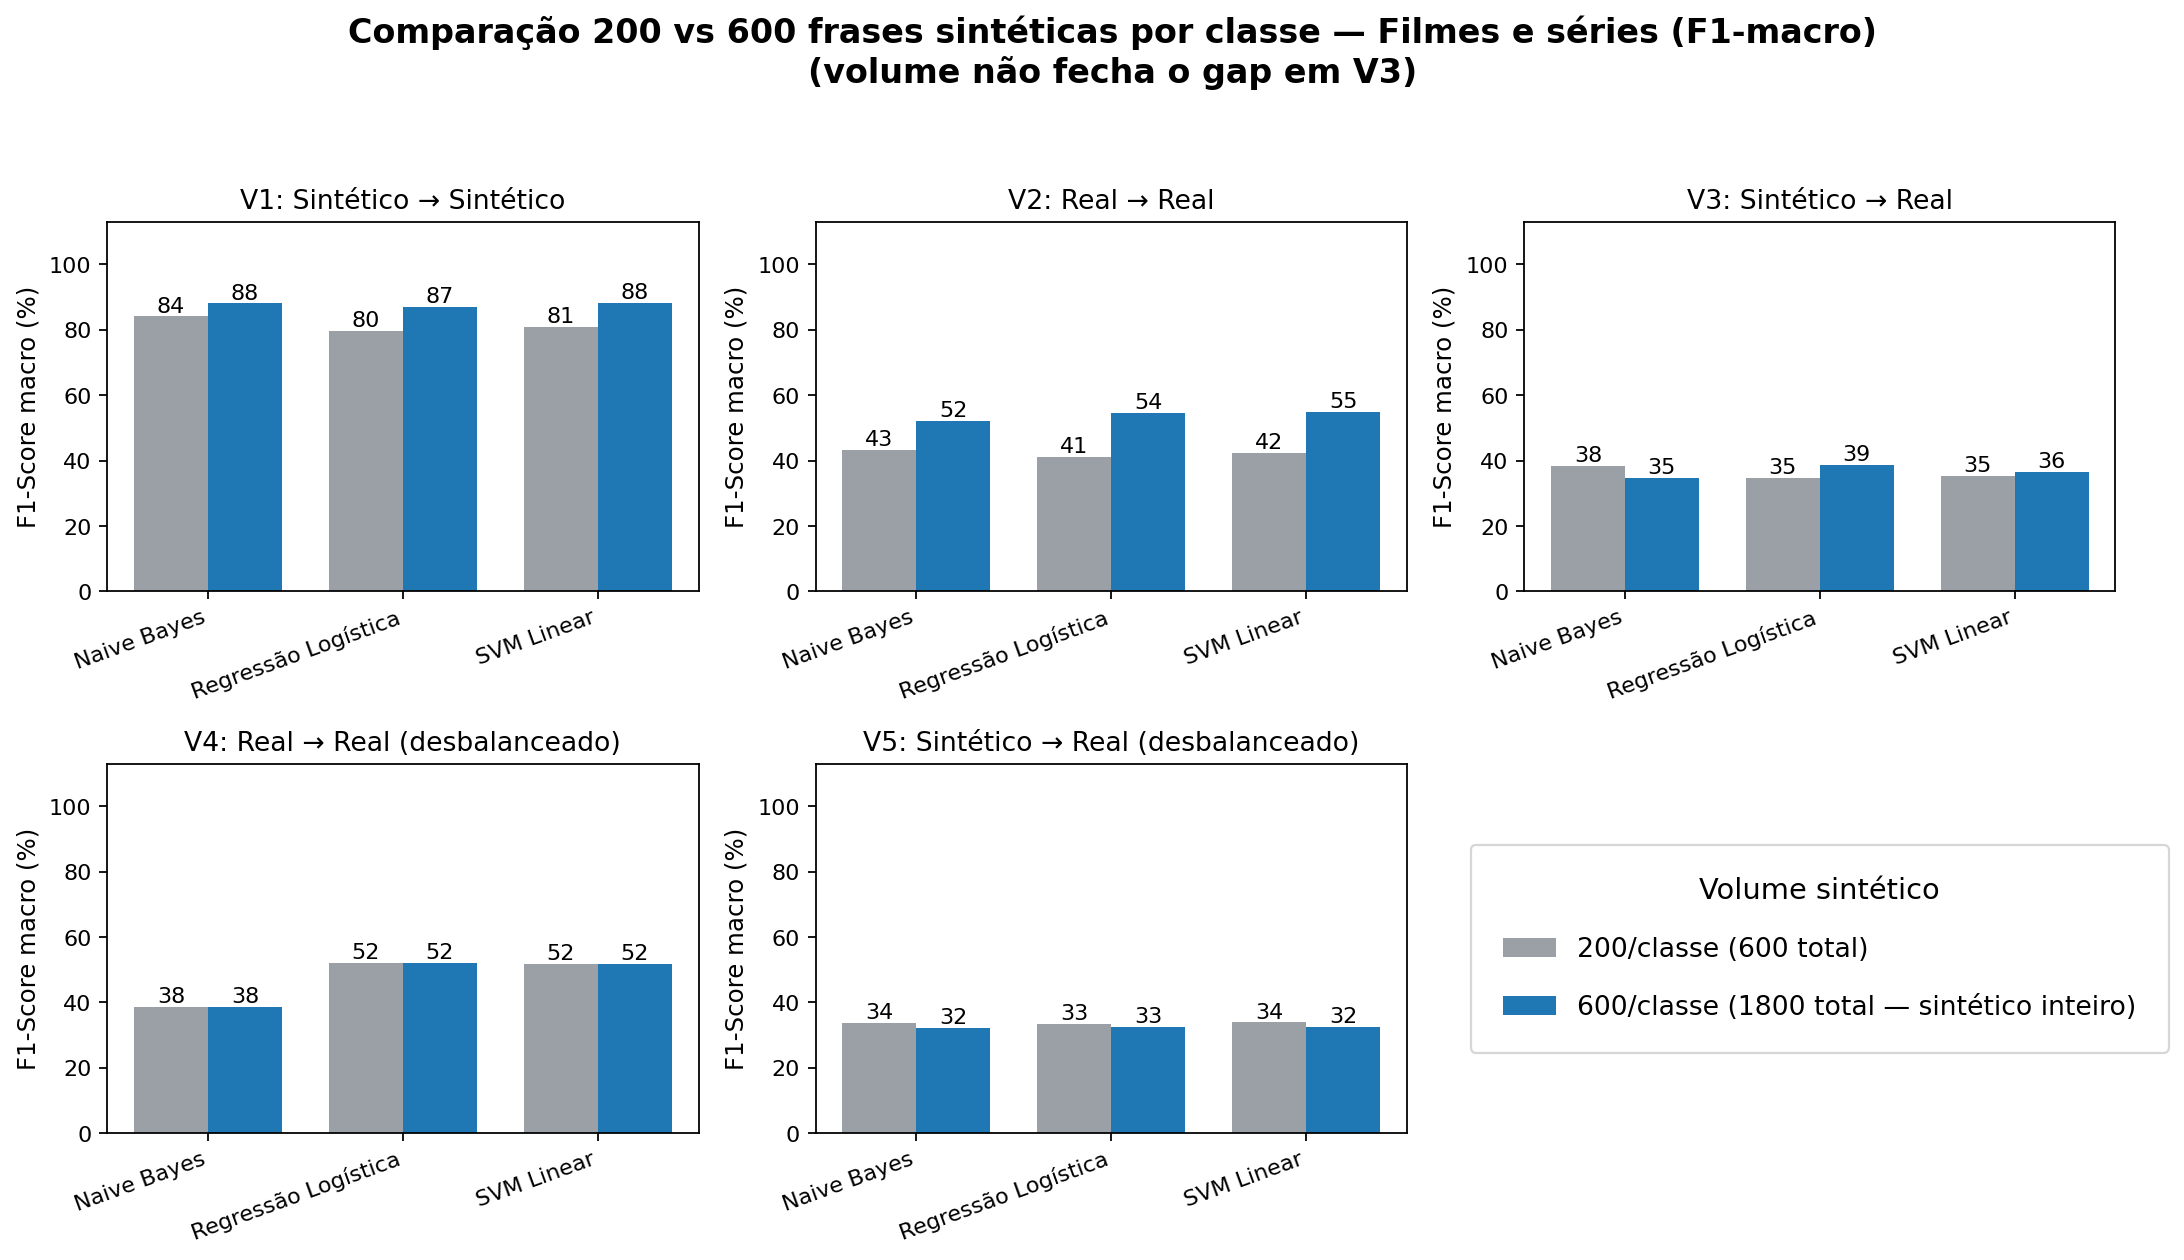
\includegraphics[width=\textwidth]{imagens/comparativo_200_vs_600_movies.png}
\caption{Comparação do desempenho em filmes com 200 vs 600 frases sintéticas por classe. Volume não fecha o gap em V3.}
\label{fig:200vs600}
\end{figure}

\subsection{Comparativo entre Nichos}

Comparando os dois nichos, apps tende a apresentar desempenho um pouco maior do que filmes em quase todas as visões. Mas a diferença mais marcante está em V5: o BERTimbau alcança 80,95\% F1 weighted em apps contra 58,95\% em filmes — uma diferença de 22 pontos. Mesmo nos modelos clássicos a diferença em V5 é de 17 a 19 pontos a favor de apps.

Essa diferença pode ser explicada pela natureza dos dois nichos. Reviews de aplicativos tendem a ser mais objetivas e técnicas — o usuário reclama de coisas concretas como travamentos, consumo de bateria ou anúncios excessivos. Esse tipo de vocabulário é mais regular e está mais próximo do que os LLMs geram naturalmente. Reviews de filmes têm narrativa, comparações com outras obras, ironia e apreciação subjetiva — uma linguagem mais distante do que o LLM produz sem instruções específicas. A consequência prática é que a viabilidade de treinar com dados sintéticos depende do nicho: pode funcionar melhor em domínios objetivos de avaliação de produto e funciona pior em domínios com linguagem mais elaborada.

\subsection{Validação Cruzada}

Como complemento, foi realizada a validação cruzada estratificada com k=5 e k=10 sobre o dataset sintético inteiro de filmes (1.798 frases) para os modelos clássicos. A Tabela~\ref{tab:cv} apresenta os resultados.

\begin{table}[h]
\centering
\caption{F1-Score (\%) com validação cruzada estratificada no dataset sintético de filmes.}
\label{tab:cv}
\begin{tabular}{lccc}
\toprule
\textbf{Modelo} & \textbf{k} & \textbf{Acurácia (\%)} & \textbf{F1-Score (\%)} \\
\midrule
Naive Bayes    & 5  & 88,82 $\pm$ 1,83 & 88,86 $\pm$ 1,82 \\
Naive Bayes    & 10 & 89,50 $\pm$ 2,15 & 89,53 $\pm$ 2,15 \\
Reg. Logística & 5  & 87,32 $\pm$ 1,43 & 87,31 $\pm$ 1,42 \\
Reg. Logística & 10 & 88,04 $\pm$ 2,42 & 88,02 $\pm$ 2,44 \\
SVM Linear     & 5  & 88,88 $\pm$ 1,33 & 88,88 $\pm$ 1,33 \\
SVM Linear     & 10 & 89,10 $\pm$ 2,49 & 89,10 $\pm$ 2,51 \\
\bottomrule
\end{tabular}
\end{table}

Os desvios padrão abaixo de 2,5\% indicam estabilidade nas estimativas — os classificadores não dependem de uma divisão particular do dataset para alcançar esses resultados. Esses valores correspondem ao cenário sintético-sintético, equivalente à visão V1, e reforçam o que foi observado nessa visão: os modelos aprendem bem o padrão dos dados sintéticos, mas isso não se traduz em bom desempenho cross-domain.


% ====================================================================
% SEÇÃO 6 — CONCLUSÃO
% ====================================================================

\section{Conclusão}
\label{sec:conclusao}

Os resultados deste trabalho mostram que dados sintéticos gerados por LLMs não constituem uma alternativa viável para treinar classificadores de sentimento destinados a uso prático. Modelos treinados exclusivamente em frases sintéticas e avaliados em reviews reais atingem no máximo 47\% de F1 weighted no nicho de filmes e 80\% no nicho de aplicativos, valores muito abaixo do patamar mínimo aceitável para qualquer aplicação que exija confiabilidade. Esse desempenho aparece de forma consistente nas cinco visões metodológicas testadas e nos cinco modelos avaliados, o que indica que a limitação não decorre de uma escolha pontual de classificador ou hiperparâmetro, mas sim de uma diferença estrutural entre o texto gerado por LLMs e as avaliações escritas por usuários reais.

A análise comparativa entre volumes de 200 e 600 frases por classe reforça essa interpretação. Triplicar a quantidade de dados sintéticos no treino mantém o desempenho cross-domain praticamente inalterado, o que mostra que a limitação observada não vem da escassez de dados, e sim da regularidade do vocabulário, da polaridade explícita e da baixa incidência de construções complexas como negação composta e ironia nas frases sintéticas. Modelos contextuais pré-treinados como o BERTimbau atenuam parte do problema, recuperando entre dez e quinze pontos percentuais sobre os classificadores baseados em TF-IDF, mas mesmo essa melhoria não chega a níveis suficientes para uso em produção.

Um aspecto metodológico relevante é o que pode ser descrito como um paradoxo de avaliação. Para calibrar e melhorar a qualidade dos dados sintéticos seria necessário compará-los com dados reais rotulados, o que torna o sintético um complemento dependente do real e não uma alternativa autônoma. Construir prompts capazes de gerar frases representativas sem nenhuma referência a dados reais é uma tarefa difícil na prática, e durante este trabalho foi observado que LLMs sem instruções específicas tendem a produzir conteúdo combinatório repetitivo, com baixa diversidade linguística. Esse comportamento sugere que a viabilidade da abordagem está condicionada à existência prévia de algum conjunto real para guiar o processo de geração.

A análise de custo também aponta na mesma direção. Em cenários onde o objetivo é classificar um volume moderado de frases, pagar diretamente uma API de LLM para realizar a classificação em modo zero-shot tende a ser mais econômico e mais assertivo do que gerar dados sintéticos, treinar um modelo próprio e arcar com a infraestrutura necessária. A combinação de custo da API para geração, tempo de desenvolvimento, infraestrutura de treinamento e desempenho final inferior torna o caminho sintético desfavorável para a maior parte das aplicações comuns. A abordagem mantém algum valor em situações específicas, como cenários com restrições de privacidade que impeçam o envio de dados a APIs externas, necessidade de inferência offline ou em dispositivos embarcados, volumes muito altos de classificação onde o custo da API se torna proibitivo, exigências de compliance que demandem modelo proprietário, ou domínios com tão pouco dado disponível que a geração sintética se torne a única opção viável.

A diferença entre os dois nichos analisados acrescenta uma nuance importante. Apps mostrou resultados consistentemente melhores que filmes nas visões cross-domain, especialmente em V5 com BERTimbau (+22 pontos). Reviews de aplicativos têm vocabulário mais regular e objetivo (problemas técnicos concretos), enquanto reviews de filmes têm linguagem narrativa mais elaborada. Isso sugere que a viabilidade de treinar com dados sintéticos depende do nicho: pode funcionar melhor em domínios de avaliação de produto e funciona pior em domínios com linguagem subjetiva extensa.

A principal contribuição deste trabalho está em demonstrar empiricamente esse conjunto de limitações e quantificá-las de forma sistemática, em dois nichos distintos e com cinco classificadores cobrindo desde modelos lineares baseados em TF-IDF até arquiteturas neurais com pretreino em larga escala. A evidência reunida permite afirmar que dados sintéticos gerados por LLMs ainda não são uma substituição prática para corpora reais em análise de sentimento em português brasileiro, mas oferecem um ponto de partida funcional para pesquisa exploratória, prototipagem inicial e cenários onde o uso de dados reais é inviável por restrições externas. Como trabalhos futuros, seria interessante investigar se técnicas de adaptação de domínio (como combinar pequena quantidade de dados reais com bastante dado sintético) conseguem fechar o gap, e estender a análise para outros nichos com graus variados de subjetividade.


\bibliographystyle{sbc}
\bibliography{referencias}

\end{document}
